\renewcommand{\vec}[1]{\textbf{#1}}

\chapter{Experimental Results}
\label{cha:experimental_results}

\section{2D Density Estimation}

To test the simple model from Section \ref{sec:simple_pc} with the discussed algorithms, so Expectation Maximization (EM), 
Gradient Descent (GD), Score Matching (SM) and Sliced Score Matching (SSM) from Sections \ref{sec:gmm_em} to \ref{sec:gmm_ssm}, we used some 
two dimensional data to perform density estimation. 

Samples from the three datasets we used can be seen in Figure \ref{fig:2d_datasets}. \\

\vspace{10pt}
\begin{figure}[H]
    \centering
    \begin{subfigure}[b]{0.4\textwidth} 
        \centering
        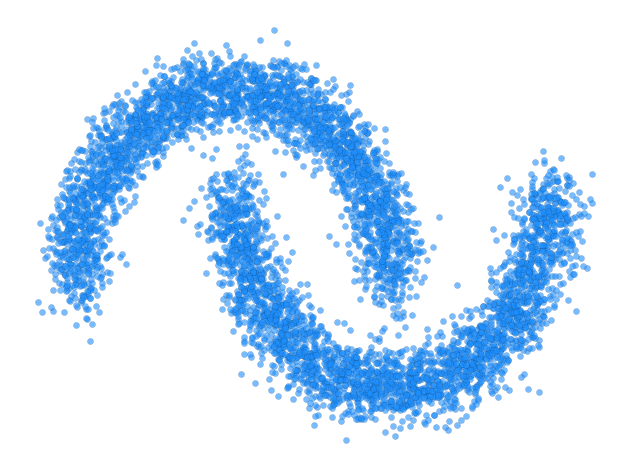
\includegraphics[width=\textwidth]{figures/halfmoons.png}
        \caption{halfmoons}
    \end{subfigure}
    \hfill
    \begin{subfigure}[b]{0.4\textwidth} 
        \centering
        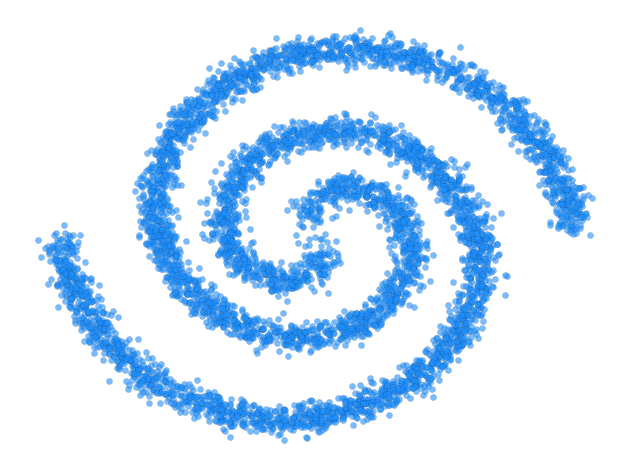
\includegraphics[width=\textwidth]{figures/spirals.png} 
        \caption{spirals}
    \end{subfigure}
    
    \vskip\baselineskip 
    \begin{subfigure}[b]{0.4\textwidth} 
        \centering
        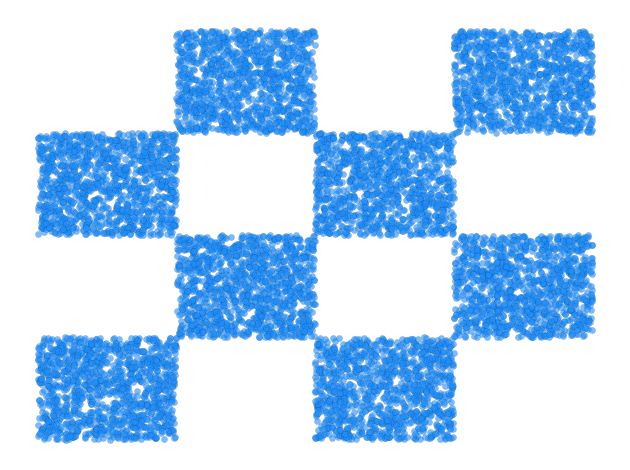
\includegraphics[width=\textwidth]{figures/board.png}
        \caption{board}
    \end{subfigure}
    
    \caption{Samples for all three datasets}
    \label{fig:2d_datasets}
\end{figure}


\subsection{Main Experiment}
\label{sec:best_results}

Here the goal was to achieve the best possible results for each algorithm on each dataset. 
For this we generated 20,000 data points for each dataset and split them evenly for training and validation. However before the training process can start, recall 
that our model is governed by the learnable parameters $\boldsymbol \pi$ (mixture weights), $\boldsymbol \mu$ (means of components) and
$\boldsymbol \Sigma$ (covariance matrices of components) that need to be initialized in some manner and the hyperparameter $K$ (mixture count) that needs to be chosen. 

As for the learnable parameters, we initialized the mixture weights $\boldsymbol \pi$ uniformly 
\[
    \boldsymbol{\pi}_k = \frac{1}{K}, \quad k = 1, 2, \dots, K
\]
the covariance matrices $\boldsymbol \Sigma$ as identity matrices of size $D \times D$ 
\[
    \mathbf{\Sigma}_k = \mathbf{I}_D, \quad k = 1, 2, \dots, K
\]
where $D$ is the dimensionality of the data and the means $\boldsymbol \mu$ by computing cluster centers of the data with the sklearn \cite{sklearn} implementation of KMeans. 

As for $K$, through some initial testing we chose three different values, namely a minimal $K$, that is needed for producing reasonable results, 
a very large $K$ from which onward there are diminishing returns and a moderate $K$ in the middle.

For the training process, recall that it is also governed by hyperparameters, namely the number of iterations $T$ for all algorithms and 
the learning rate $\eta$ for all the gradient-based algorithms (GD, SM, SSM).
To choose these parameters we fixed $K$ to one of the three chosen values and performed cross-validation by computing the validation set Log-Likelihood 
of the models with all possible remaining hyperparameter combinations and choosing the combination with the highest Log-Likelihood.

Results, more specifically Log-Likelihood, estimated densities and samples for all datasets and all values of $K$ can be seen in the following three pages.  

\newpage
\begin{figure}[H]
    \centering
    \makebox[\textwidth][c]{\hspace*{-1cm} 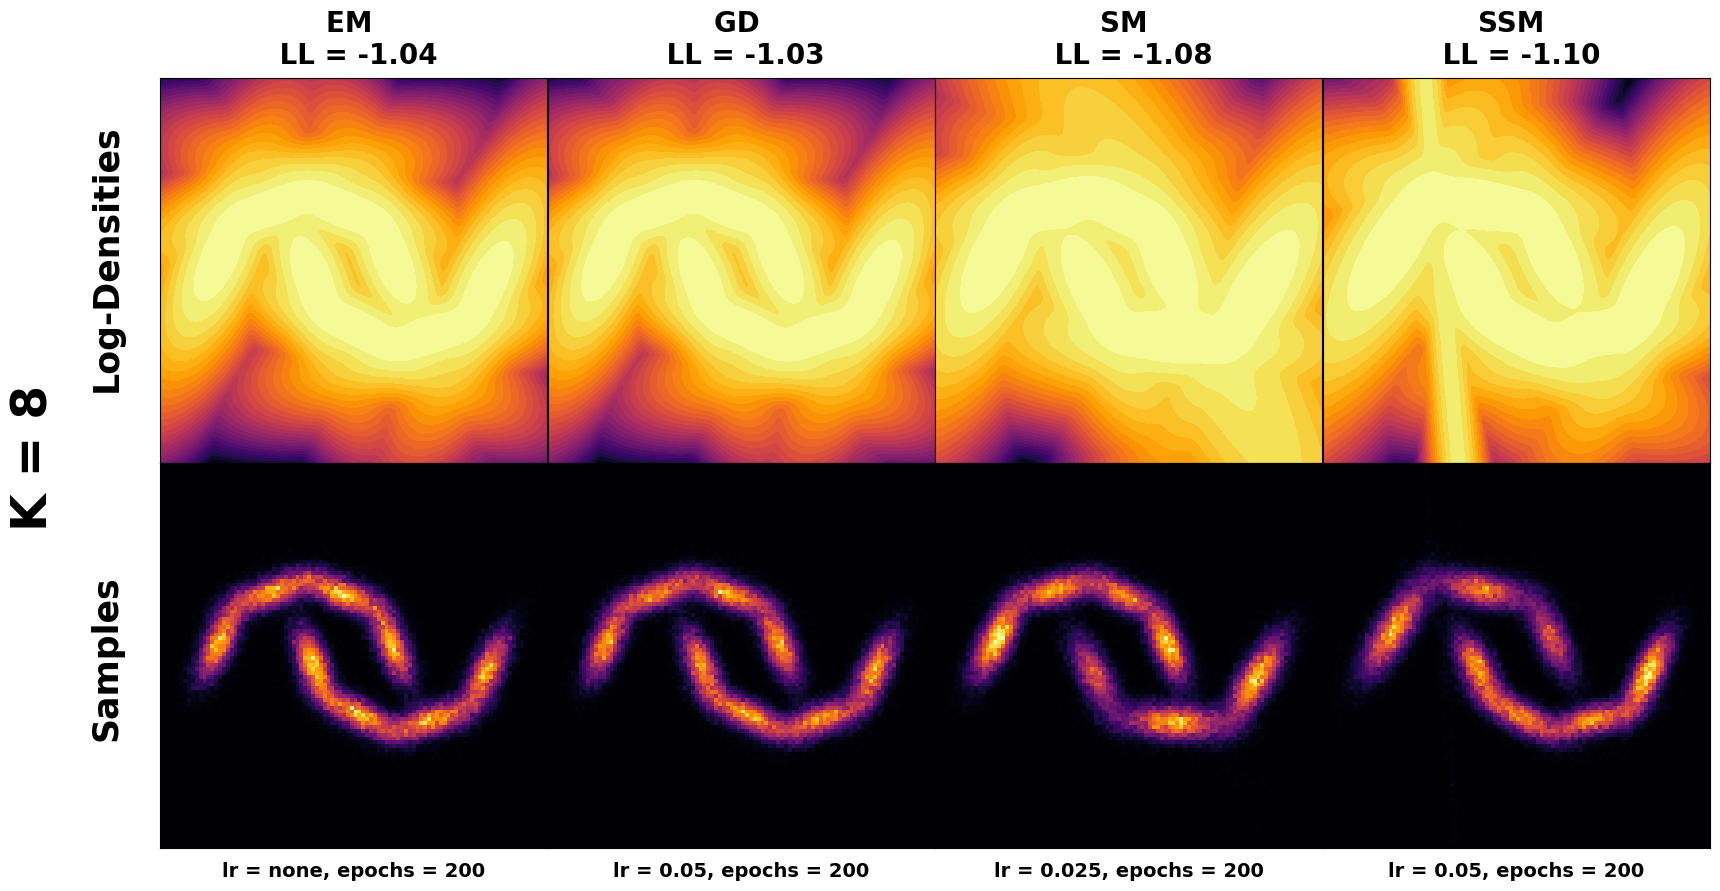
\includegraphics[width=0.9\textwidth]{figures/halfmoons/halfmoons_8.png}}
    \vskip 5pt
    \makebox[\textwidth][c]{\hspace*{-1cm} 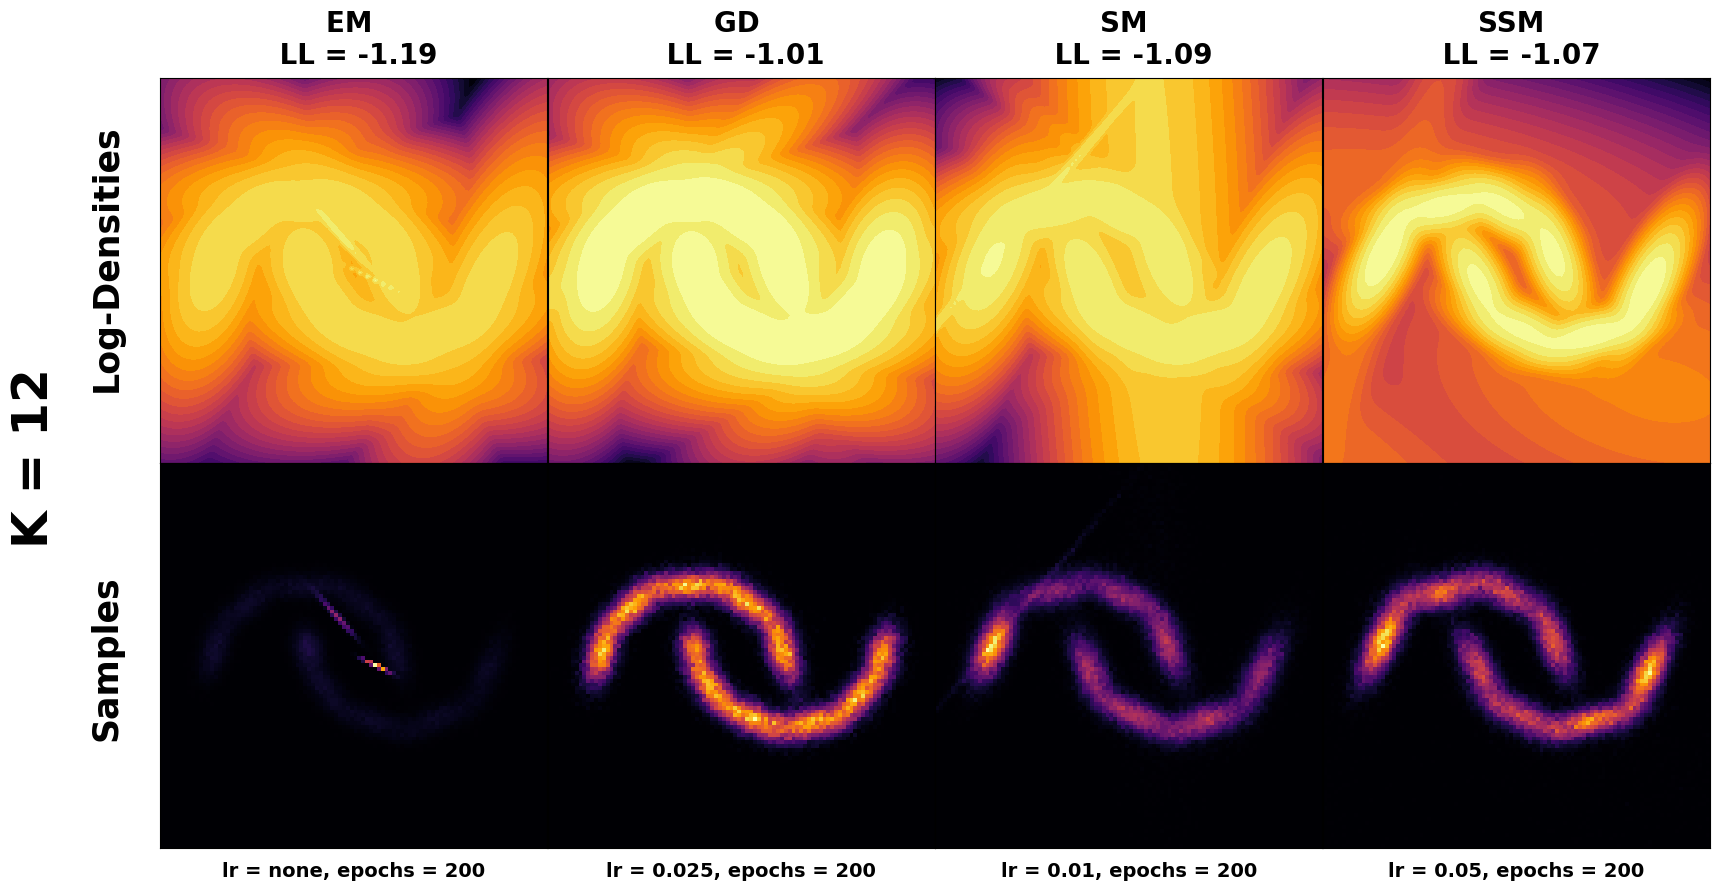
\includegraphics[width=0.9\textwidth]{figures/halfmoons/halfmoons_12.png}}
    \vskip 5pt
    \makebox[\textwidth][c]{\hspace*{-1cm} 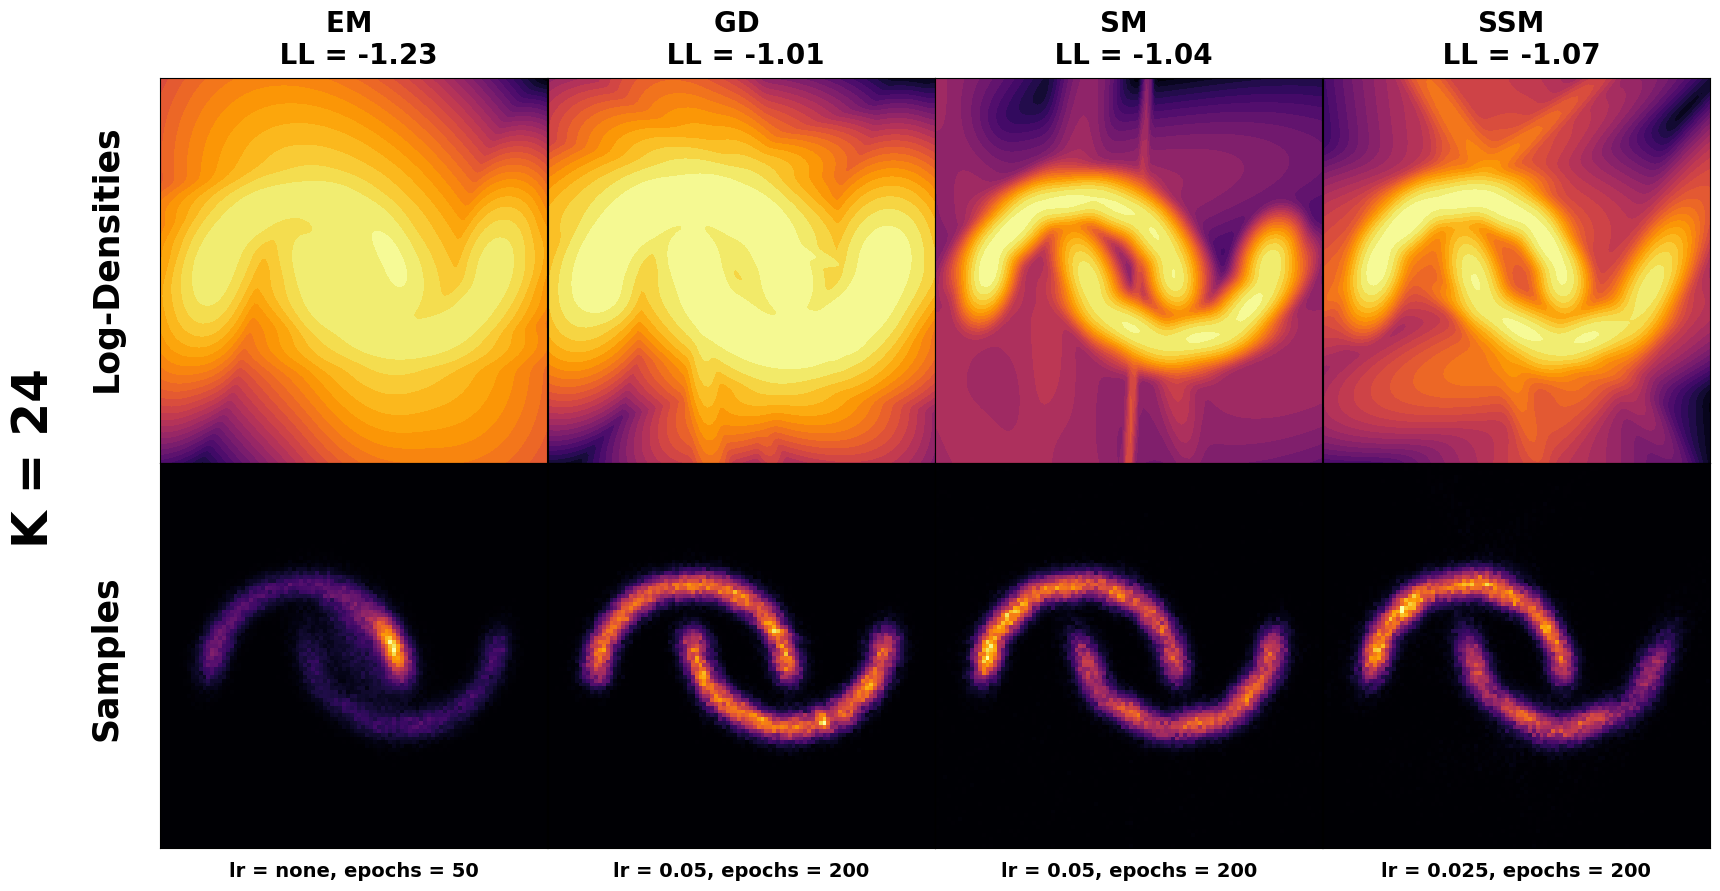
\includegraphics[width=0.9\textwidth]{figures/halfmoons/halfmoons_24.png}}
    \caption{Densities and Samples for the halfmoon dataset}
    \label{fig:exp_moons}
\end{figure}
\newpage
\begin{figure}[H]
    \centering
    \makebox[\textwidth][c]{\hspace*{-1cm} 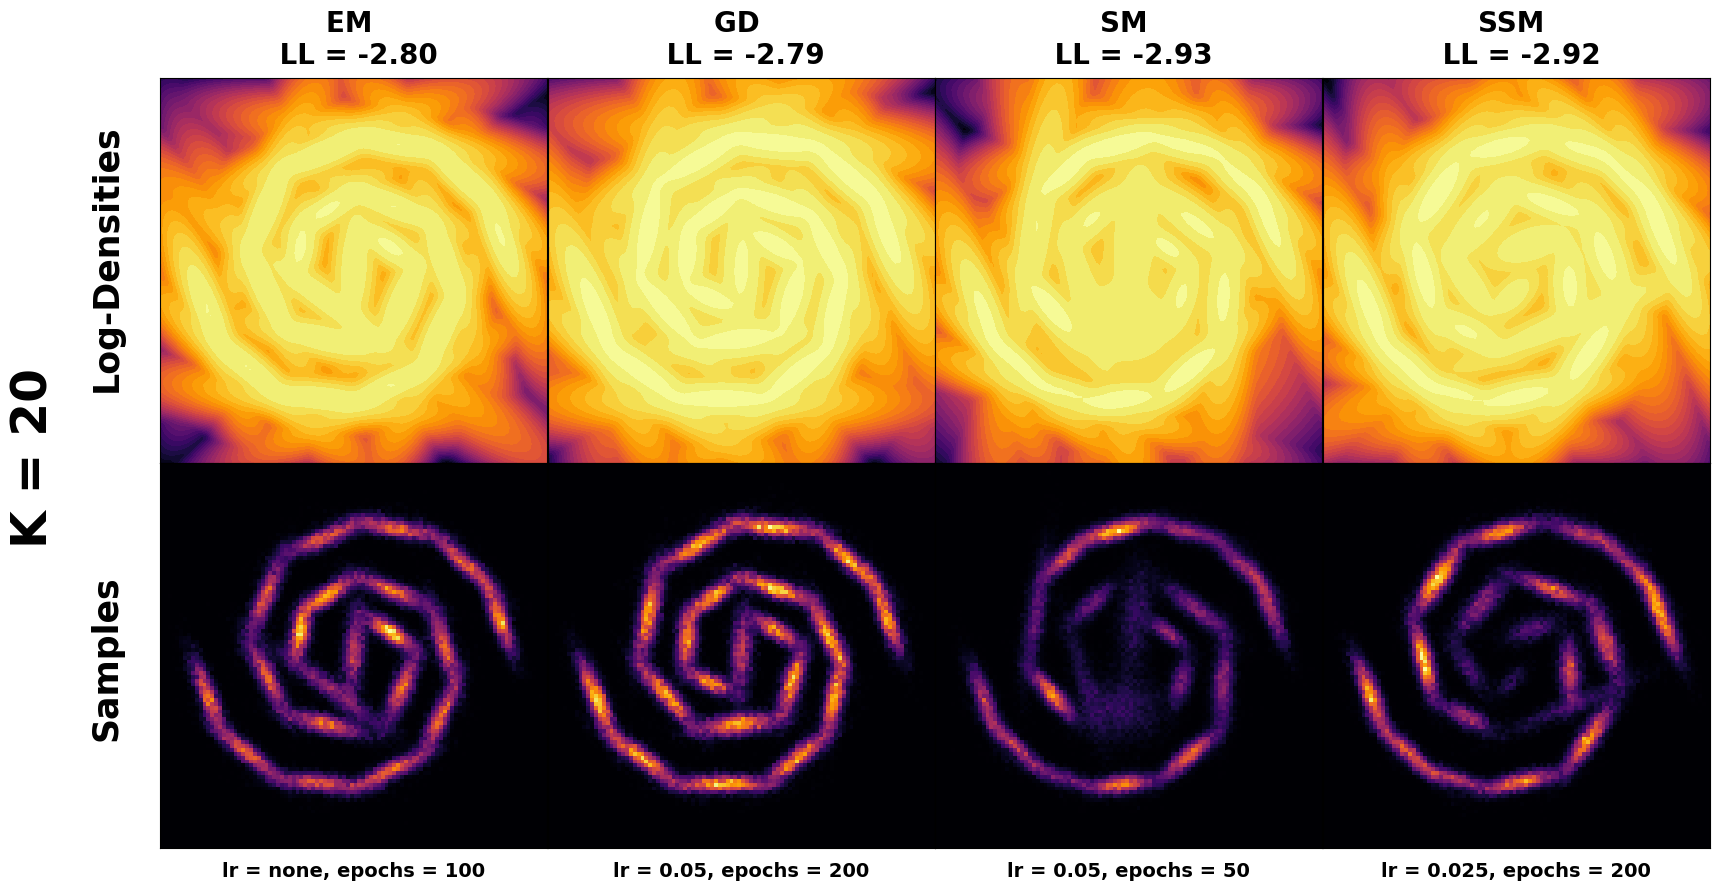
\includegraphics[width=0.9\textwidth]{figures/spirals/spirals_20.png}}
    \vskip 5pt
    \makebox[\textwidth][c]{\hspace*{-1cm} 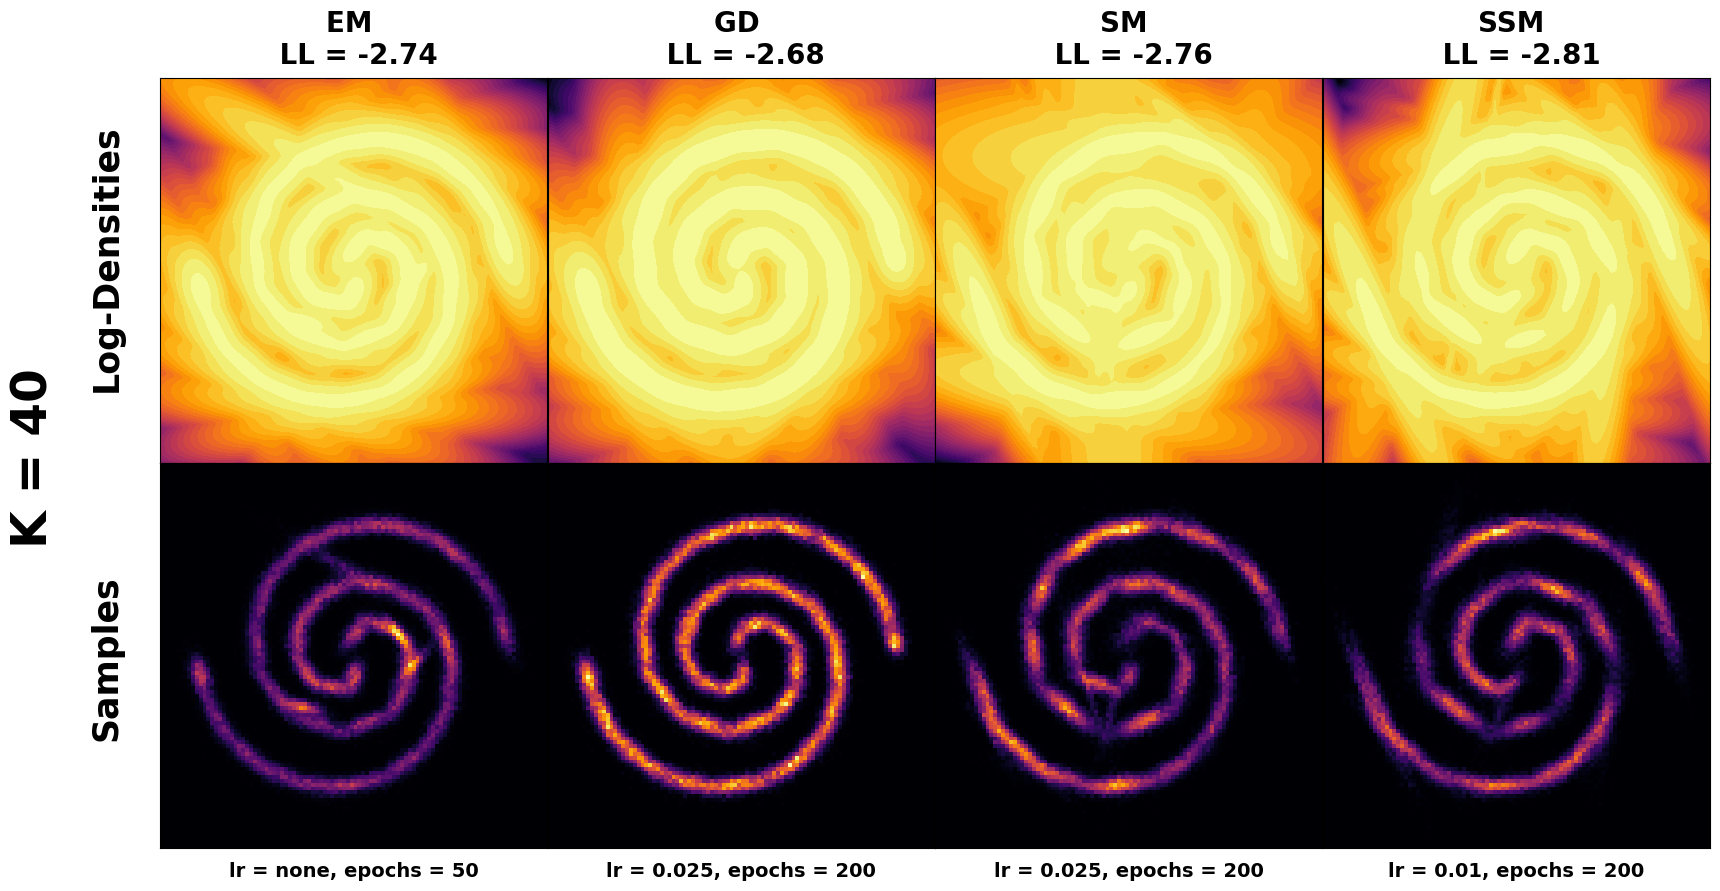
\includegraphics[width=0.9\textwidth]{figures/spirals/spirals_40.png}}
    \vskip 5pt
    \makebox[\textwidth][c]{\hspace*{-1cm} 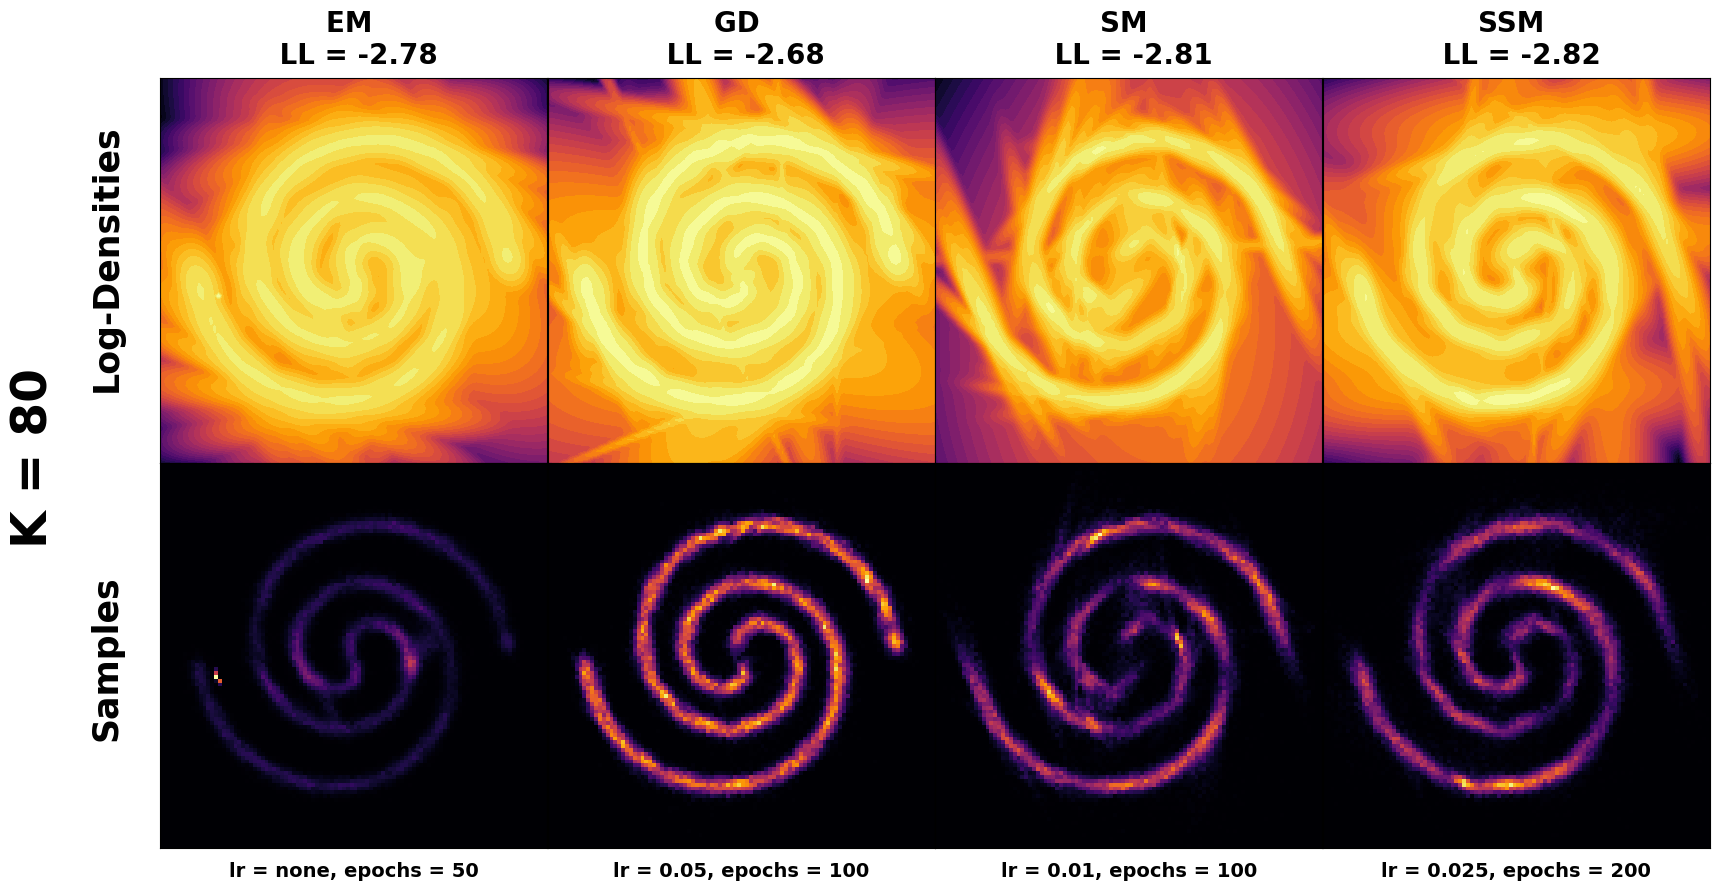
\includegraphics[width=0.9\textwidth]{figures/spirals/spirals_80.png}}
    \caption{Densities and Samples for the spirals dataset}
    \label{fig:exp_moons}
\end{figure}
\newpage
\begin{figure}[H]
    \centering
    \makebox[\textwidth][c]{\hspace*{-1cm} 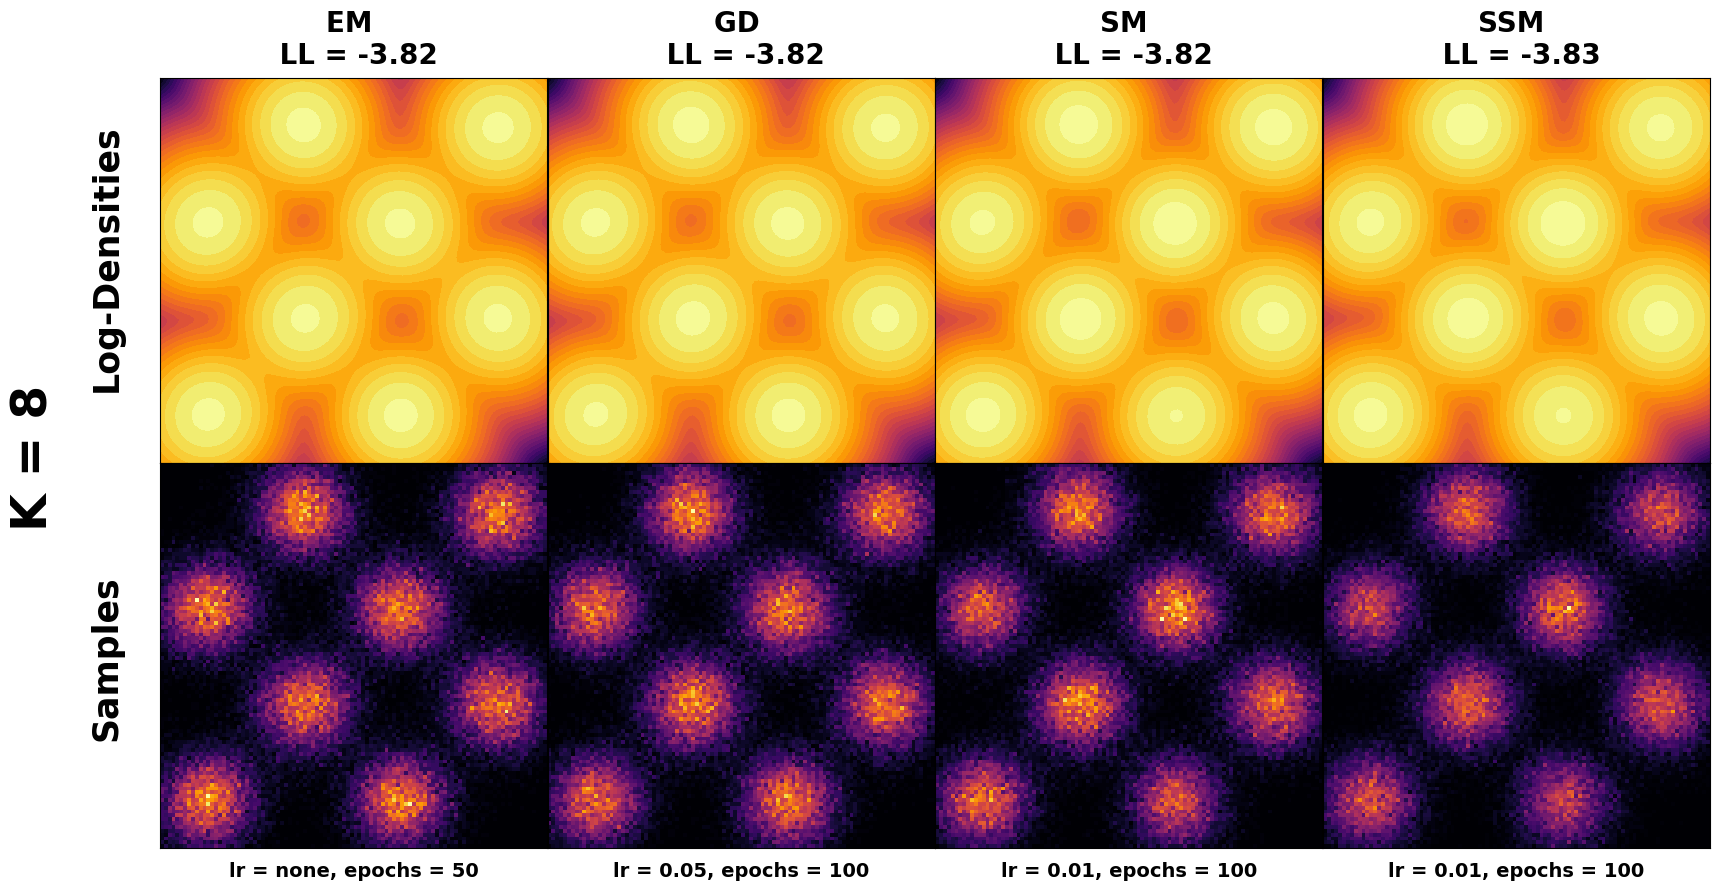
\includegraphics[width=0.9\textwidth]{figures/board_8.png}}
    \vskip 5pt
    \makebox[\textwidth][c]{\hspace*{-1cm} 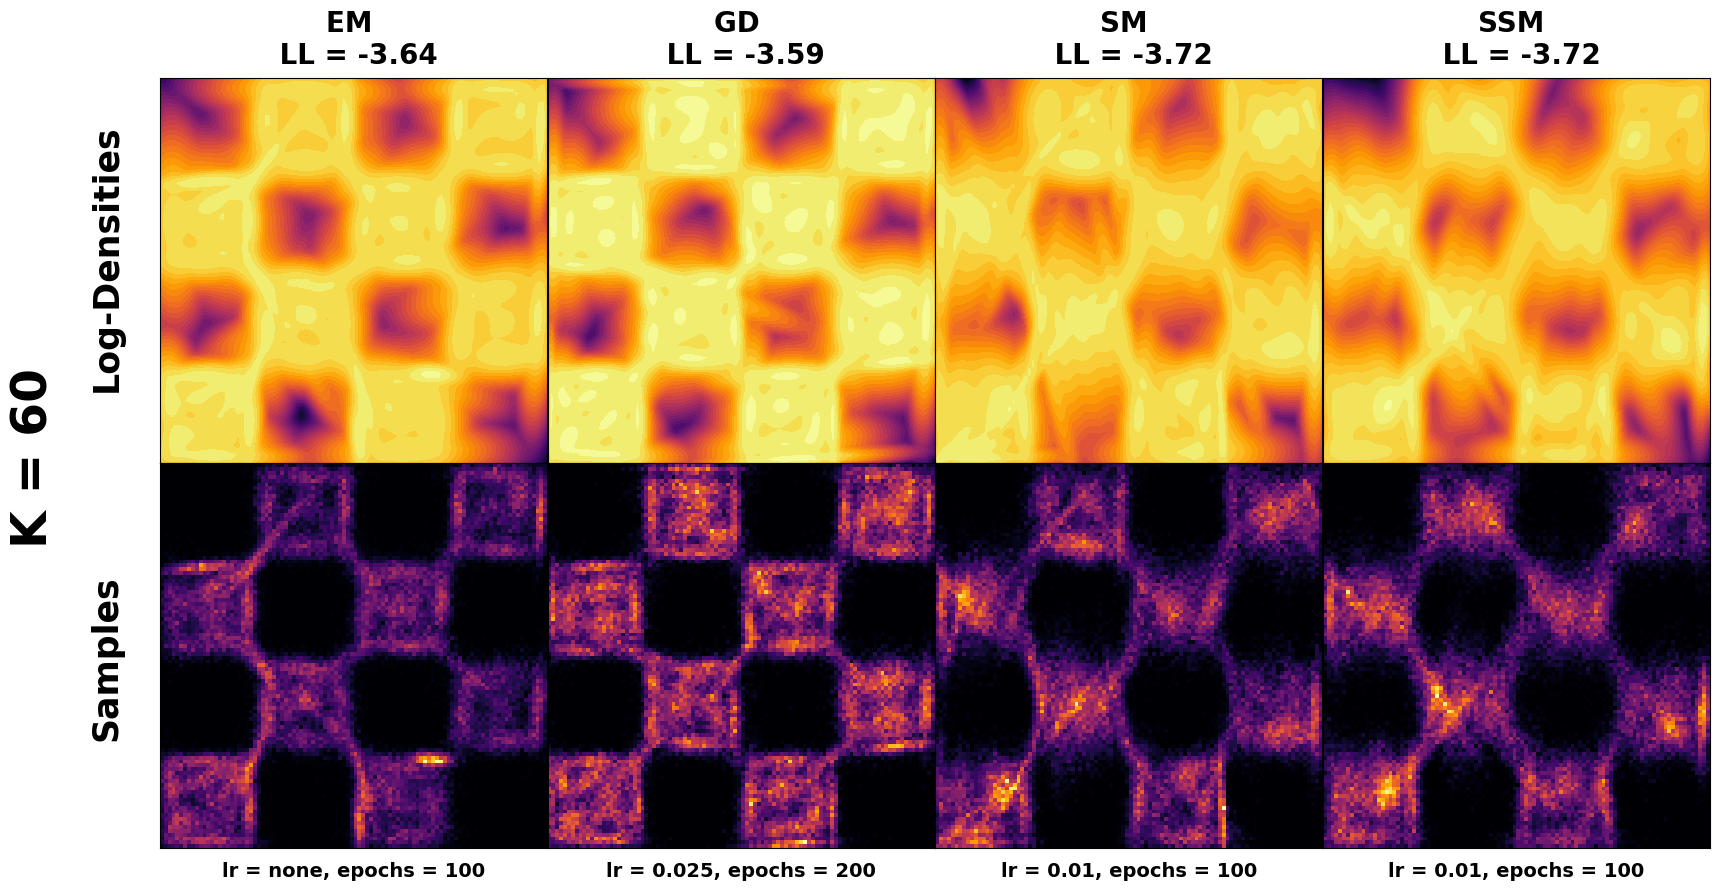
\includegraphics[width=0.9\textwidth]{figures/board_60.png}}
    \vskip 5pt
    \makebox[\textwidth][c]{\hspace*{-1cm} 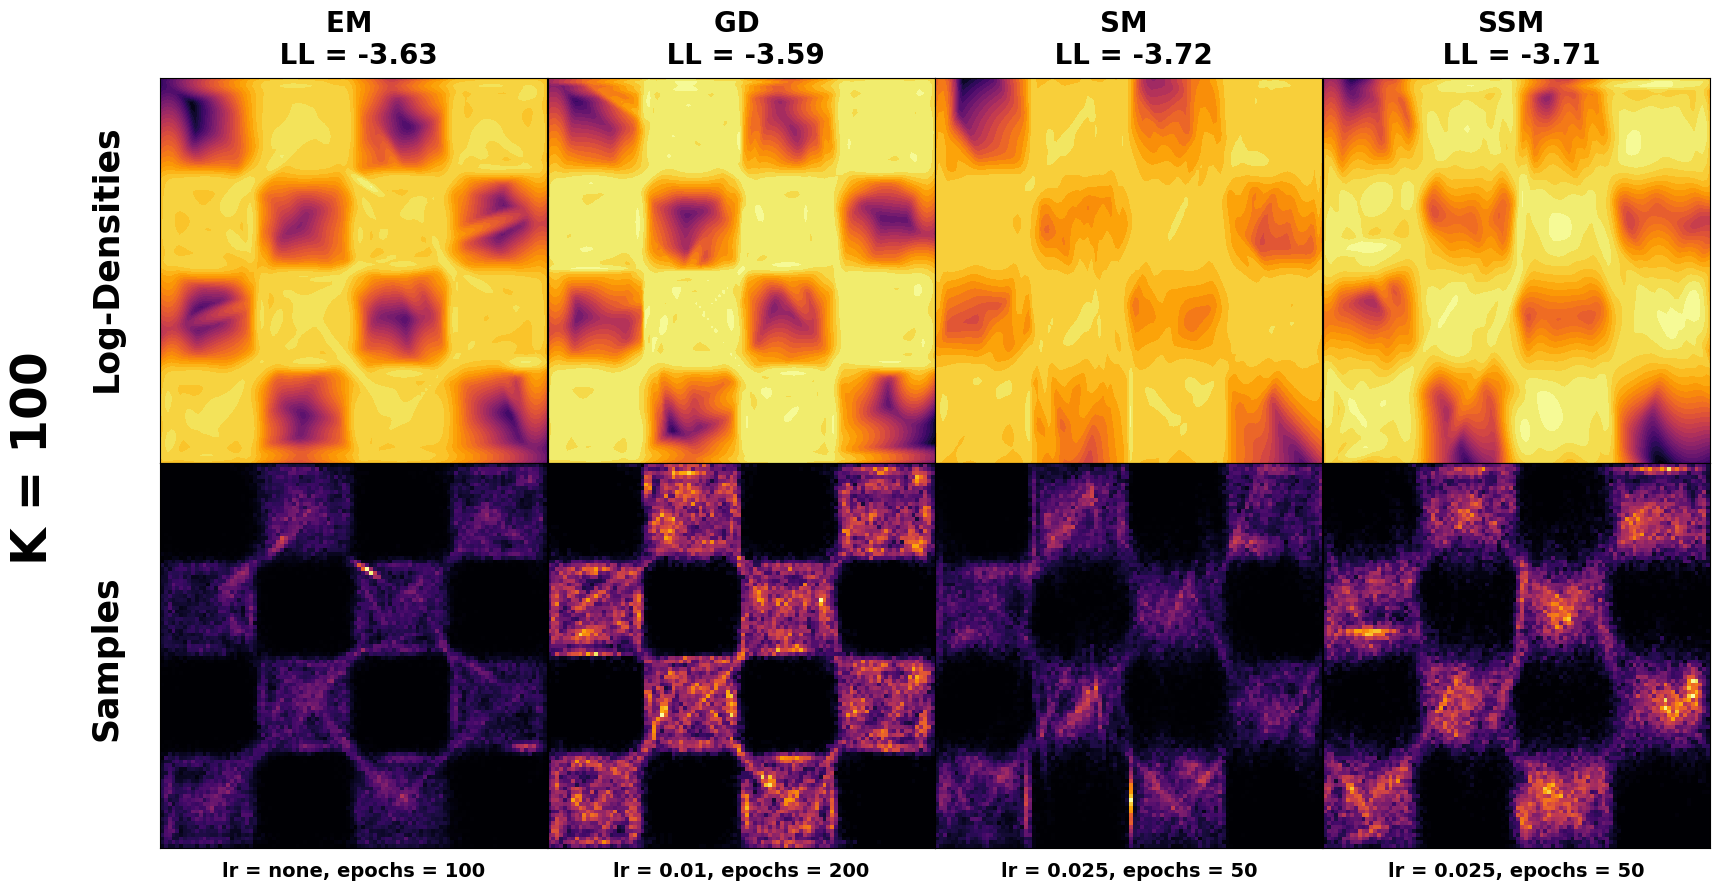
\includegraphics[width=0.9\textwidth]{figures/board_100.png}}
    \caption{Densities and Samples for the board dataset}
    \label{fig:exp_moons}
\end{figure}
\newpage

\subsection{Further Analysis}
\label{sec:2d_exp2}

\subsubsection{Training Time}

To gain further insight in how the learning process differs for each algorithm we chose a dataset and a set of hyperparameters
where all algorithms perform somewhat similar and analyzed the Negative Log-Likelihood (NLL) over Training Iterations. 
Estimated density and samples and now also the mentioned training curve can be seen in Figure \ref{fig:halfmoons_10_logp}. Because all algorithms except Sliced Score Matching are deterministic, we did multiple runs ($10$) for SSM and plotted the mean value 
with the standard deviation shaded. 

\begin{figure}[H]
    \centering
    \makebox[\textwidth][c]{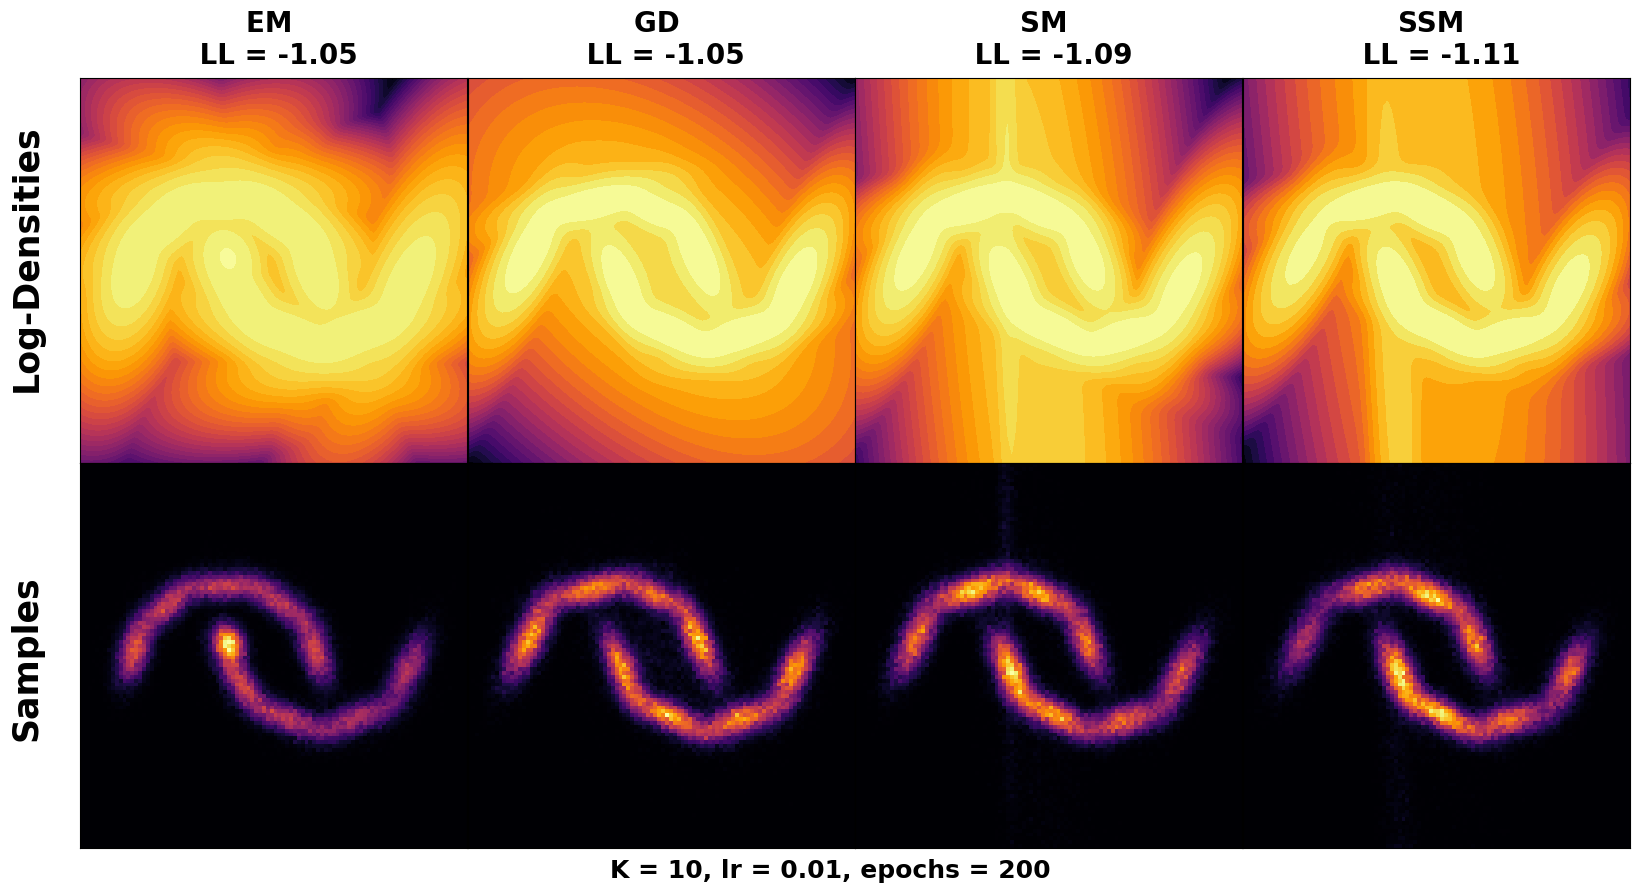
\includegraphics[width=0.8\textwidth]{figures/halfmoons/10_kmeans.png}}
    \makebox[\textwidth][c]{\hspace{-0.4cm} 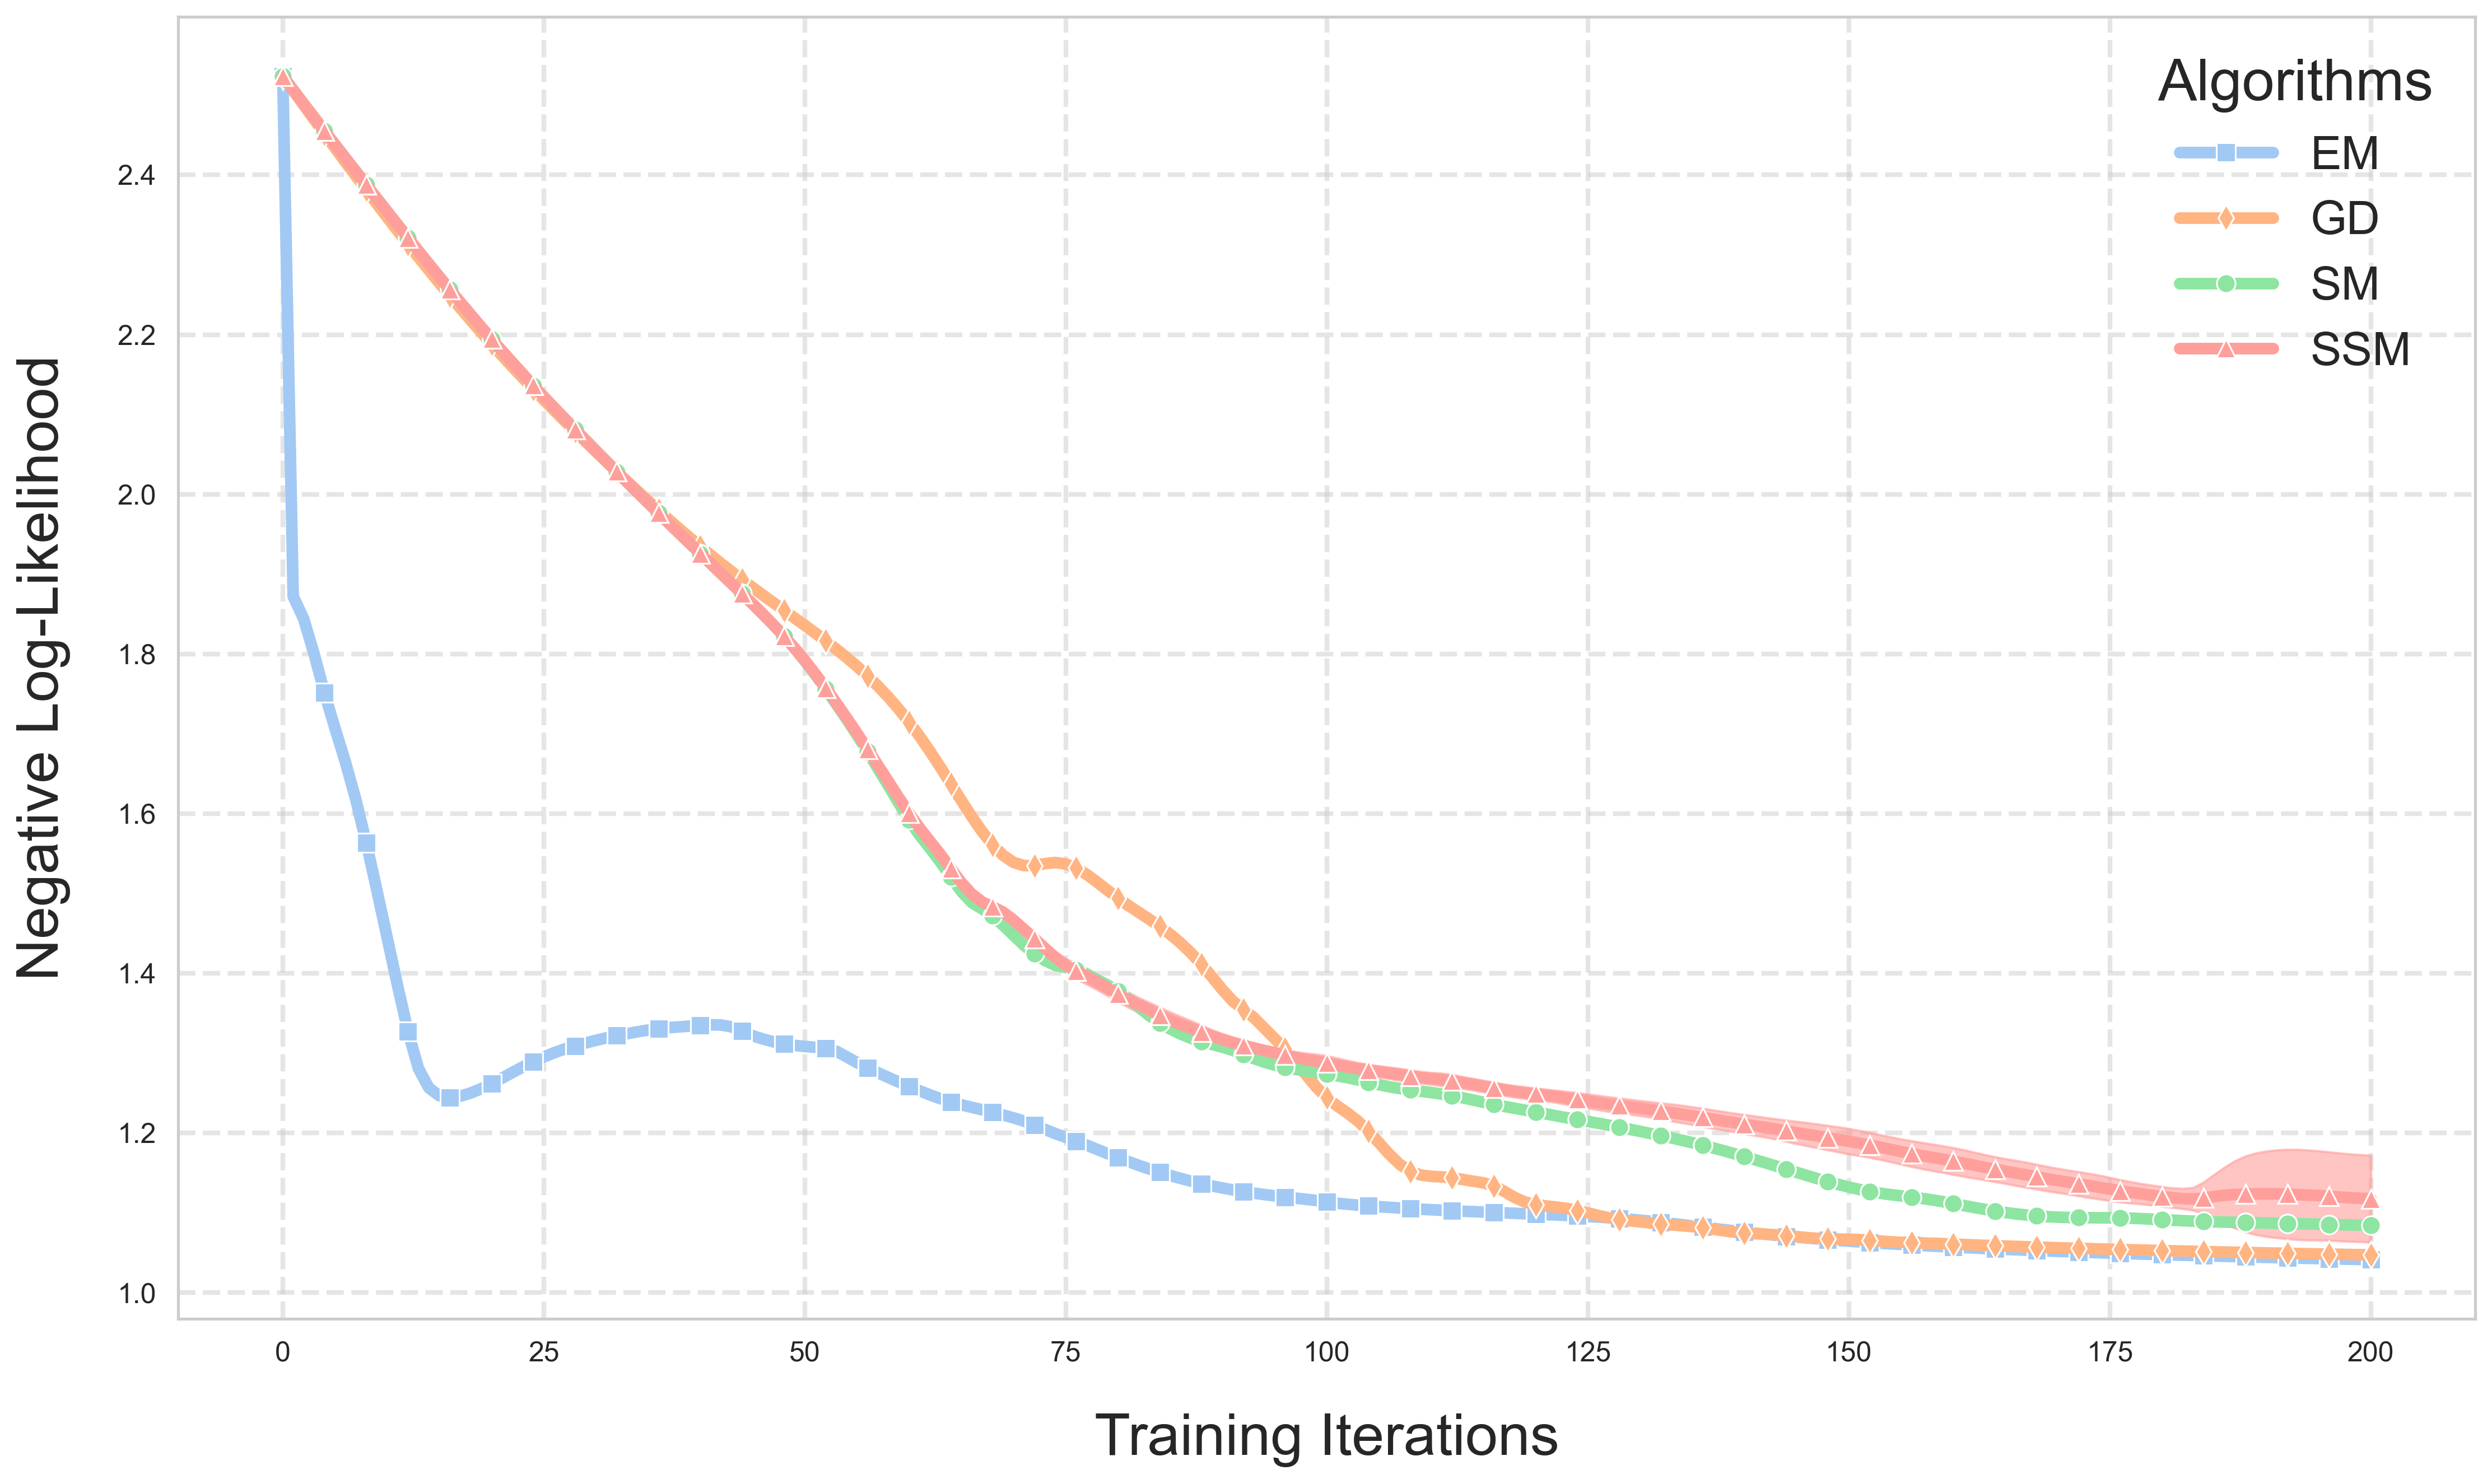
\includegraphics[width=0.9\textwidth]{figures/halfmoons/10_kmeans_logp.png}}
    \caption{Densities, Samples and NLL over Training Iterations}
    \label{fig:halfmoons_10_logp}
\end{figure}

First, we see that on average SSM performs very similar to SM (usually a little worse), which 
given that SSM is an approximation of SM, can be expected. Sometimes the stochastic nature of SSM can also 
by sheer luck yield better results. Note that when increasing the number of slices, which were $1$ for all 
experiments up until now, we saw that SSM increasingly gives a better approximation of SM.

Also clearly noticeable is that EM appears to learn the fastest and all the gradient-based algorithms
behave quite similarly. This was similar for all other datasets and hyperparameter configurations as well. 
However note that in the Figures above, we are only looking at NLL over Epochs, so we are not accounting for the 
duration of a single epoch. When running all algorithms for a specific amount of time, the differences increase considerably. 

\begin{figure}[H]
    \centering
    \makebox[\textwidth][c]{\hspace{-0.4cm} 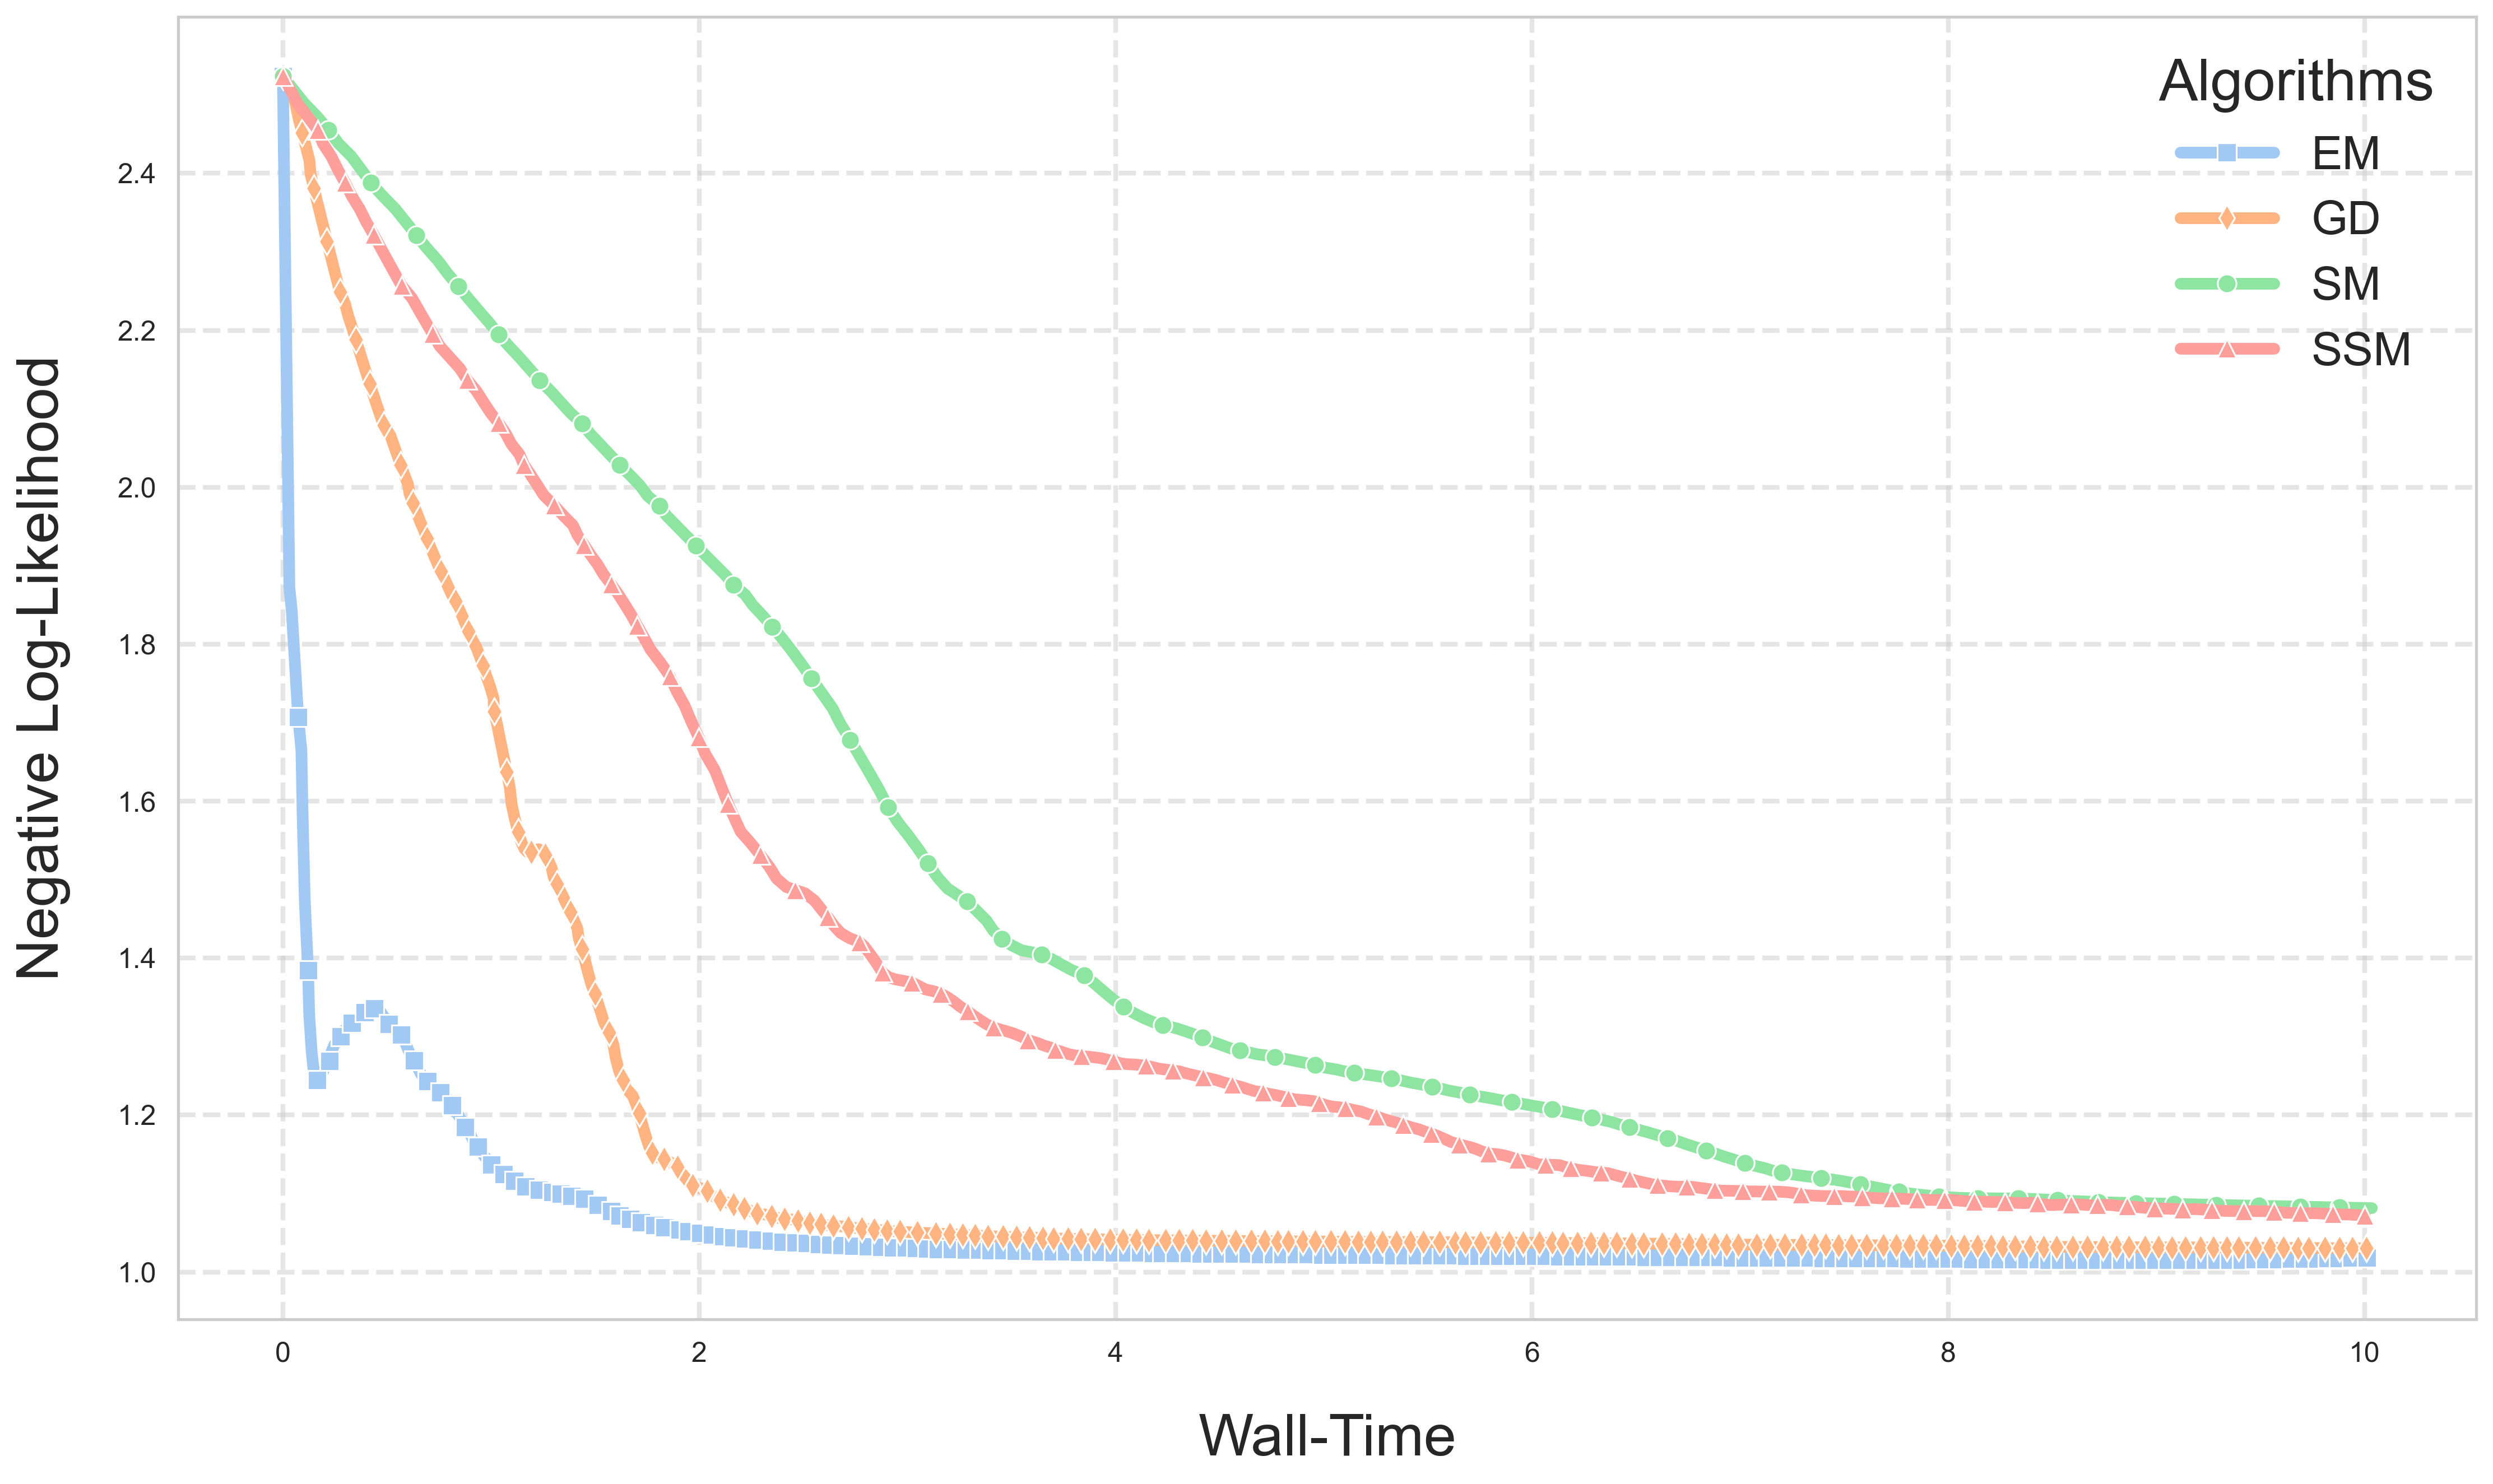
\includegraphics[width=0.9\textwidth]{figures/halfmoons/wall_time.png}}
    \caption{NLL over Time}
    \label{fig:spirals_30_kmeans}
\end{figure}

EM and GD appear considerably faster than their Score Matching alternatives, in fact while GD on average only takes 
around $1.1$ times as long as EM, SSM takes around twice as long and SM around $2.5$ times as long.

\subsubsection{Initialization}
\label{sec:2d_exp3}

Another point we wanted to examine was the initialization of the learnable parameters. 
With our data it is quite straightforward to initialize the means, which up to now has been done with KMeans, but this is not always the case.
Also initializing the weights uniformly conveniently makes a lot of sense with our data, however the initialization of both these 
parameters can be problematic and has to be done randomly quite often. \\
Therefore we also analyzed how each algorithm 
behaves when these parameters are initialized randomly. 

To initialize the means we draw $K$ random data points from our training data and 
to initialize the weights we just draw random numbers from $0$ to $1$ and normalize them so they sum to one.

\begin{figure}[H]
    \centering
    \begin{subfigure}[b]{0.49\textwidth} 
        \centering
        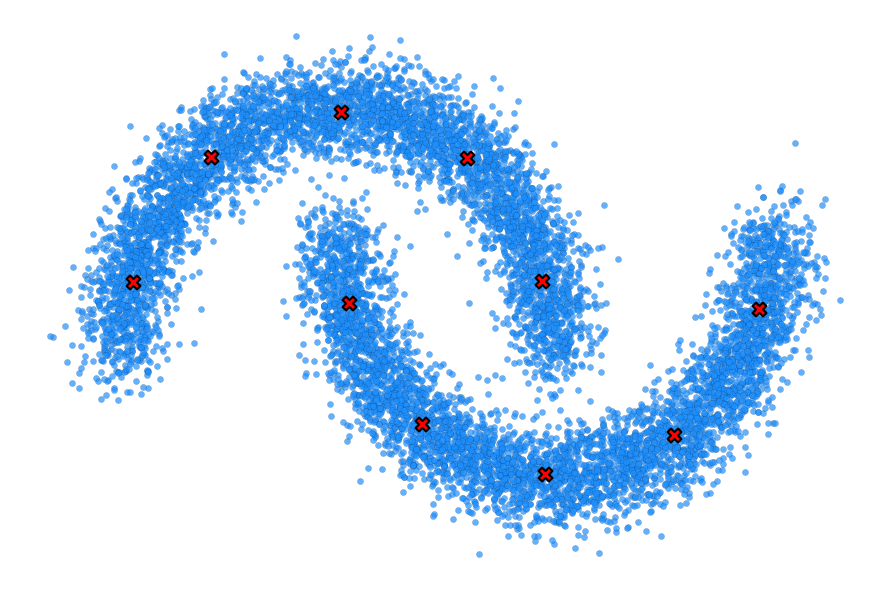
\includegraphics[width=\textwidth]{figures/halfmoons/10_kmeans_data.png}
        \caption{KMeans}
    \end{subfigure}
    \begin{subfigure}[b]{0.49\textwidth} 
        \centering
        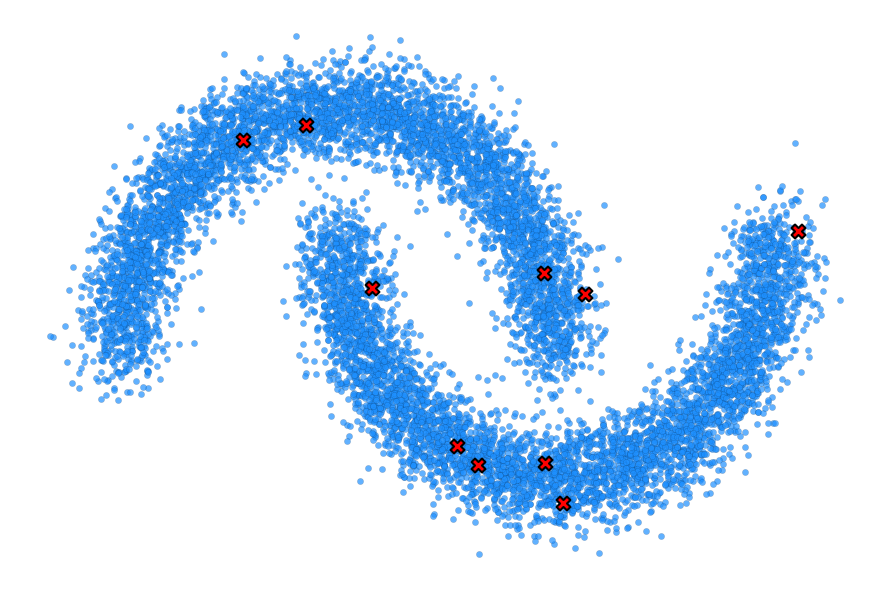
\includegraphics[width=\textwidth]{figures/halfmoons/10_random1_data.png} 
        \caption{Random}
    \end{subfigure} 
    \caption{KMeans vs. Random Initialization of means}
    \label{fig:kmeans_vs_rand}
\end{figure}

In Figure \ref{fig:halfmoons_10_random_logp} the mean Log-Likelihood and standard deviation over $10$ runs with random initialization in each run can be seen. 

\begin{figure}[H]
    \centering
    \makebox[\textwidth][c]{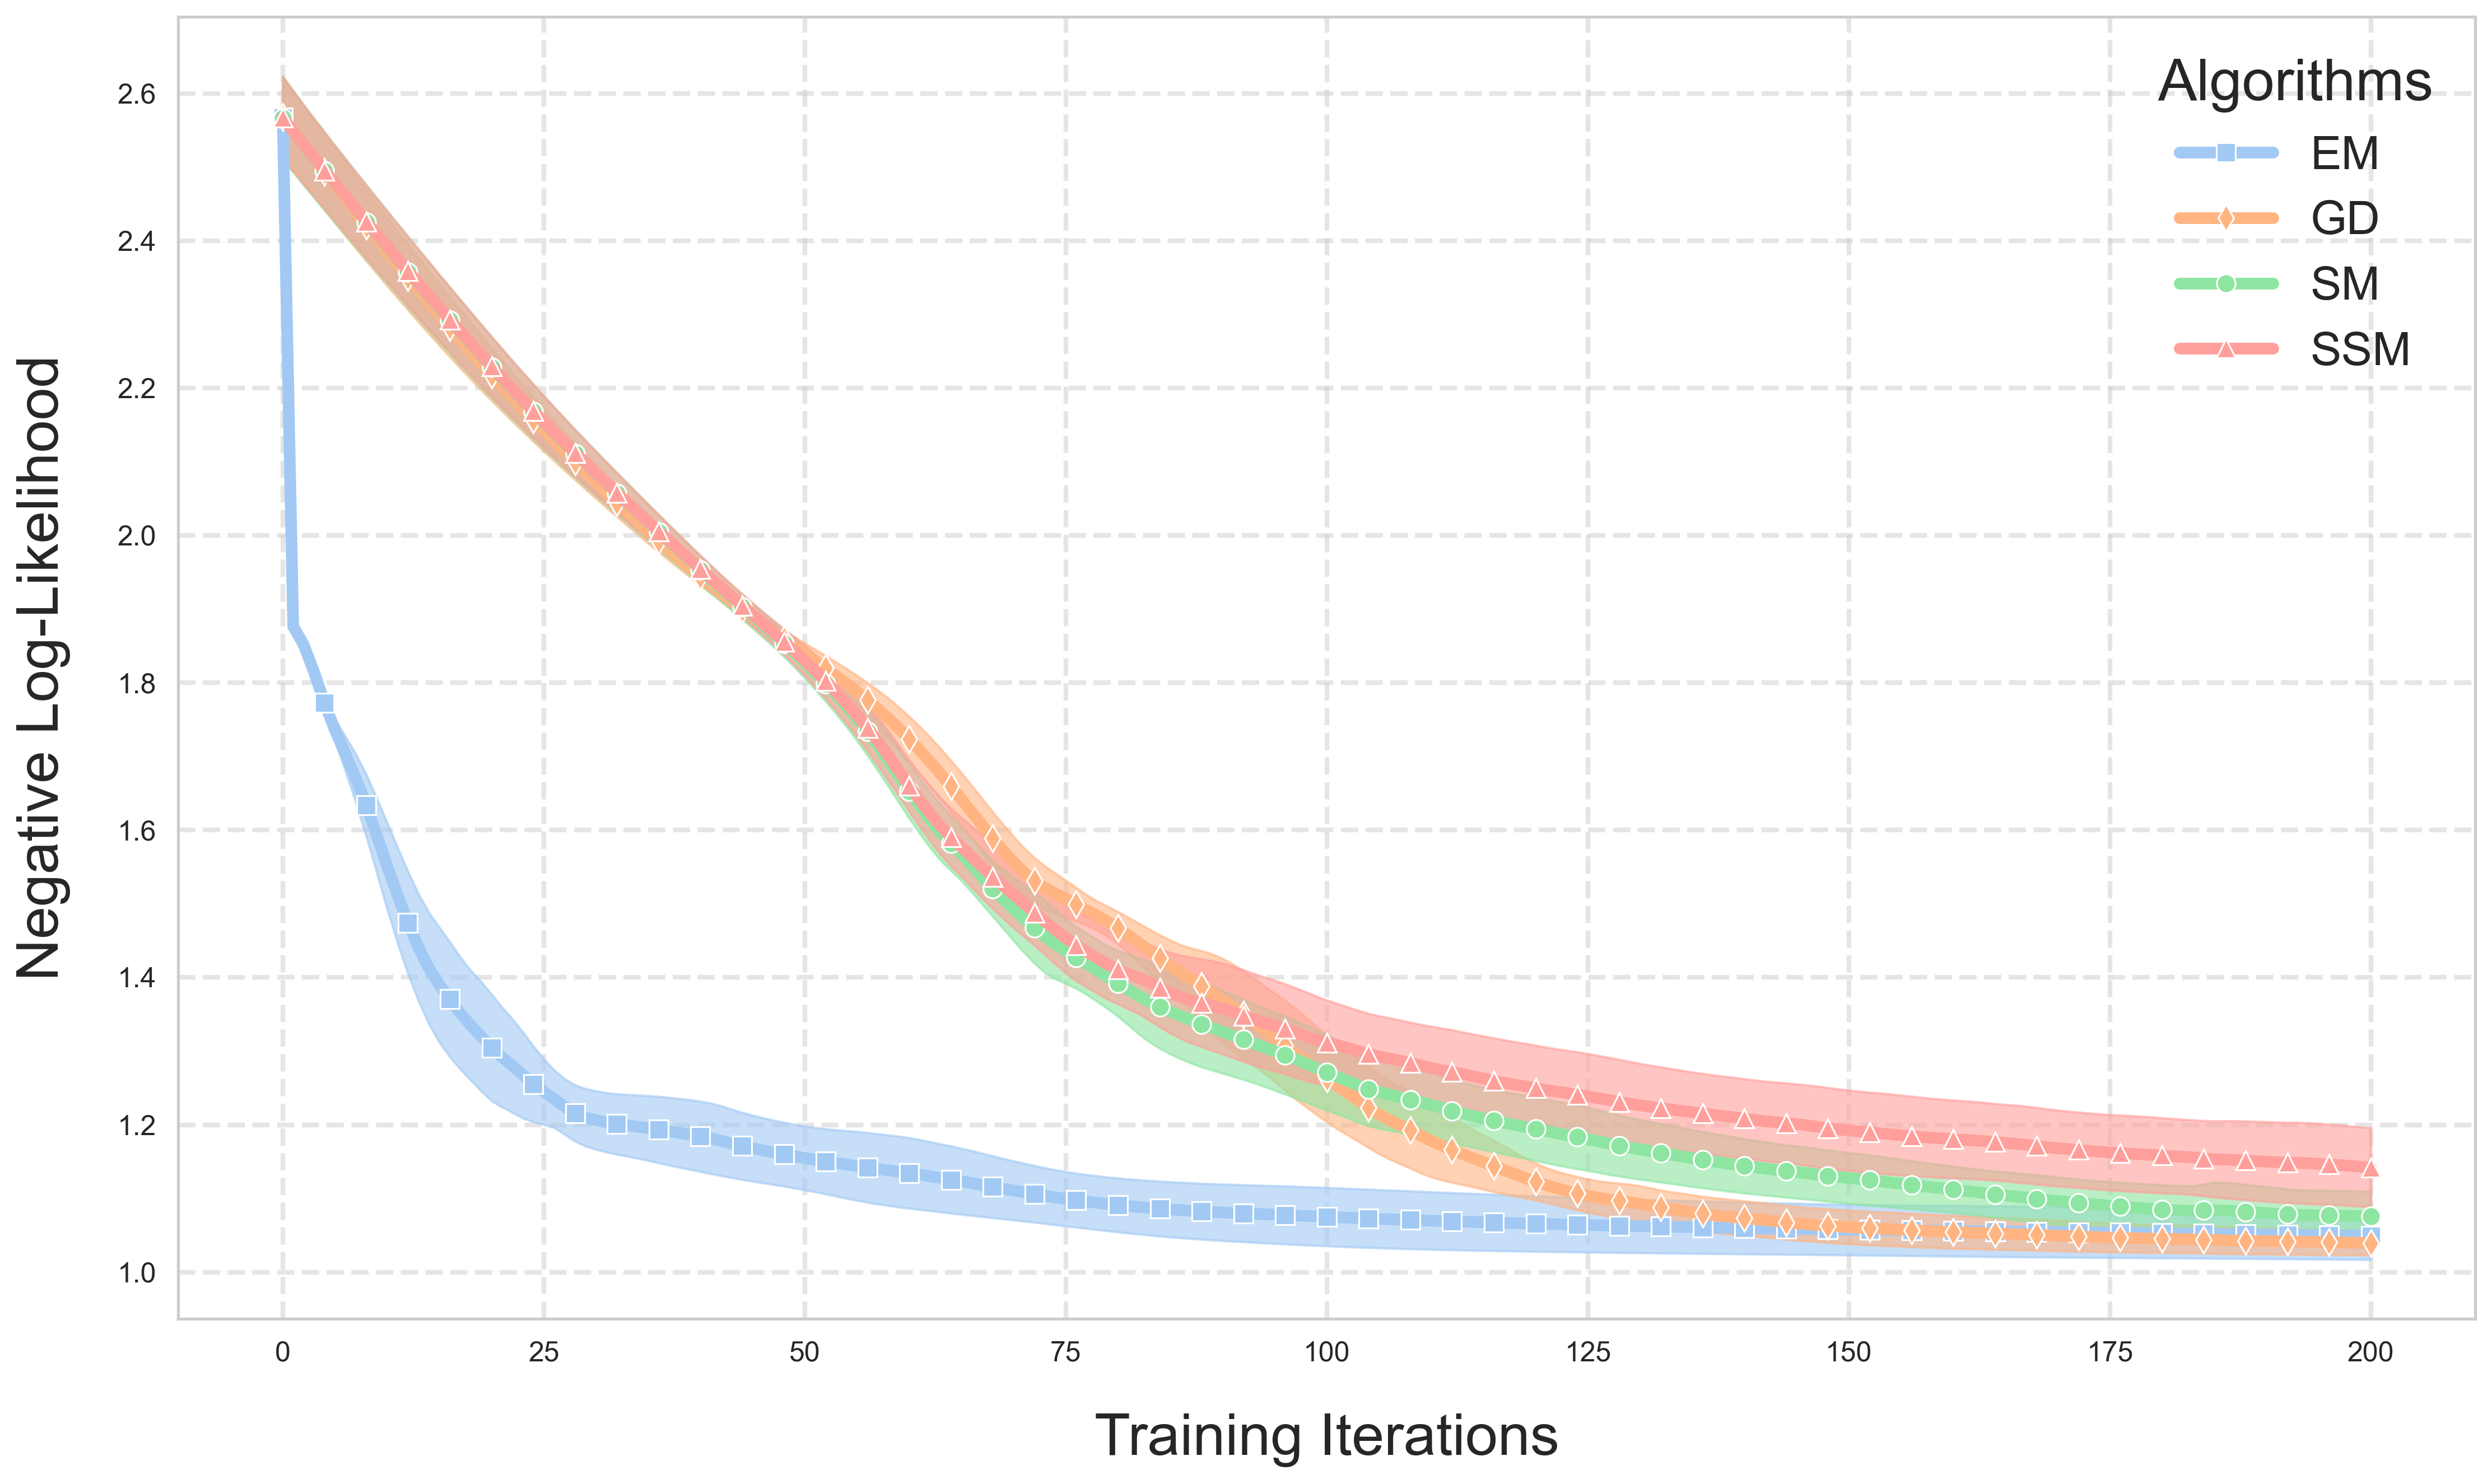
\includegraphics[width=0.9\textwidth]{figures/halfmoons/10_random_logp.png}}
    \caption{Negative Log Likelihood over Epochs with random parameter initialization}
    \label{fig:halfmoons_10_random_logp}
\end{figure}

On this simple dataset it appears that random initialization performs relatively similar to the KMeans initialization when comparing with the NLL over Epochs curve from Figure \ref{fig:halfmoons_10_logp}. For some concrete results (Densities and Samples) refer to the Appendix \ref{sec:app_halfmoons_rand}.
We repeated Experiments \ref{sec:2d_exp2} and \ref{sec:2d_exp3} for the spirals dataset, results can be found in Appendix \ref{sec:app_spirals}.

\section{Generative Image Modelling}

To train a before mentioned EinsumNetwork \cite{einsum} with our targeted algorithms, we used the provided demo-file for the MNIST \cite{mnist} dataset (\texttt{demo\_mnist.py}) and included 
our algorithms. MNIST is a dataset of handwritten digits (from 0 to 9) and quite popular for image modelling tasks.
Note that, since training already took quite long, we left out exact Score Matching and only focused on Sliced Score Matching. 

\begin{figure}[H]
    \centering
    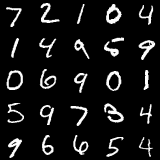
\includegraphics[width=0.4\textwidth]{figures/einsum/mnist/[]_ground_truth.png}
    \caption{Samples of MNIST}
\end{figure}

\subsection{Single Class Training}
\label{sec:exp_mnist_single}

Here the goal is to produce the best possible samples on single class of MNIST.

We left the model related hyperparameters as they were provided in the framework and only tuned the training specific hyperparameters 
(iterations and learning rate for gradient based algorithms and only iterations for EM) to find the best samples for each algorithm. 

We found that, while EM gave quite good samples after only around 10 iterations, SGD and SSM required much longer to converge. 
More precisely, we saw that training SSM or SGD with an already moderately high learning rate
of 0.01, needed around 200 iterations to produce good results, which of course increases more if we set a lower learning rate.
We provide a graph of samples at specific epochs on MNIST class 7 for all algorithms in Figure \ref{fig:mnist_epochs}.\\ 

\begin{figure}[H]
    \centering
    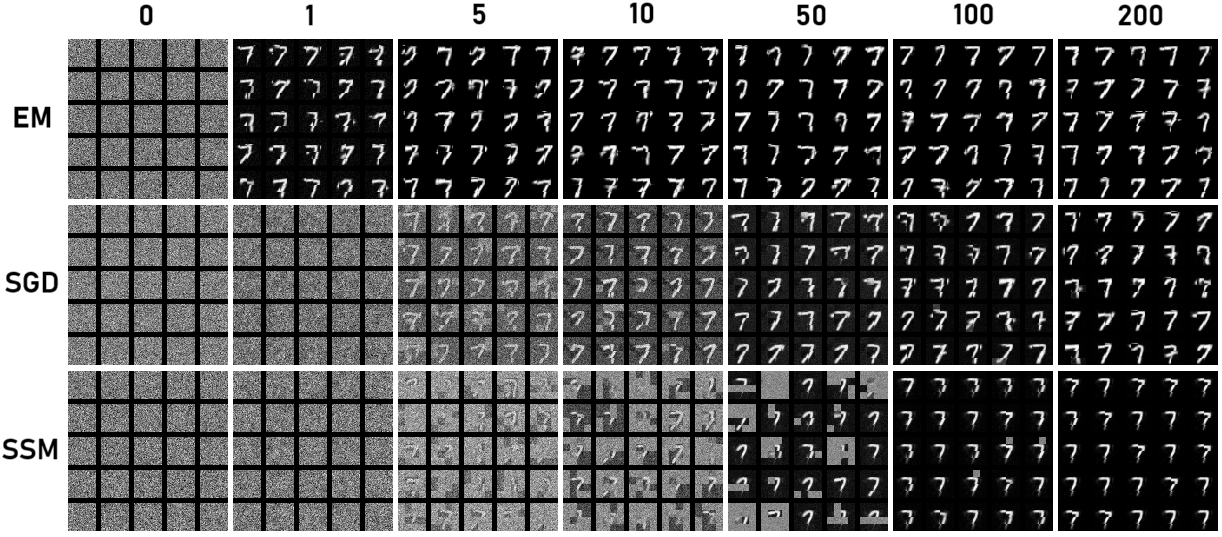
\includegraphics[width=0.8\textwidth]{figures/einsum/mnist/epoch_comparison.png}
    \caption{Samples over epochs for different training algorithms}
    \label{fig:mnist_epochs}
\end{figure}

Although increasing the learning rate further mostly worked for SGD, SSM saw vanishing or exploding gradients after some iterations and thus was
not able to properly finish. Even applying gradient clipping did not really solve this. 

Therefore the best way to train an EinsumNetwork using SSM we could find is to start with a relatively 
high learning rate of 0.2 or 0.1 and use learning rate decay to decrease it over time. Although
this could further be specifically tuned for each different MNIST digit, we find that training for 
20 iterations using an initial learning rate of 0.2 and decaying it with a factor of 0.5 every 5 epochs 
and additionally using gradient clipping with a threshold of 1.0 was the most practical approach for all classes.
This approach also improved the SGD results further.

We trained with each algorithm for 20 iterations and used the described approach for SGD and SSM, on three different classes of MNIST. 
Negative Log Likelihood (NLL) and samples can be seen in the figures below.
For results on FashionMNIST we refer to to Appendix \ref{sec:app_fashionmnist}. \\

On a side note, this setup resulted in $204146$ learnable parameters in the EinsumNetwork. For comparison the most 
complex 2D model we used with $100$ mixture components had $700$ learnable parameters. 

\begin{figure}[H]
    \centering
    \begin{subfigure}[b]{0.24\textwidth}
        \centering
        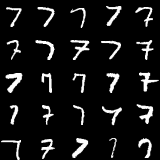
\includegraphics[width=\textwidth]{figures/einsum/mnist/[7]_ground_truth.png}
        \caption{Ground Truth}
    \end{subfigure}
    \begin{subfigure}[b]{0.24\textwidth}
        \centering
        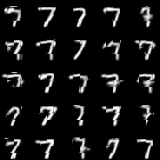
\includegraphics[width=\textwidth]{figures/einsum/mnist/[7]_EM.png}
        \caption{EM (LL: -11576)}
    \end{subfigure}
    \begin{subfigure}[b]{0.24\textwidth}
        \centering
        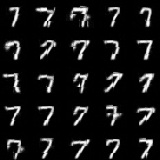
\includegraphics[width=\textwidth]{figures/einsum/mnist/[7]_SGD.png} 
        \caption{SGD (LL: -12972)}
    \end{subfigure}
    \begin{subfigure}[b]{0.24\textwidth}
        \centering
        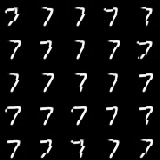
\includegraphics[width=\textwidth]{figures/einsum/mnist/[7]_SSM.png}
        \caption{SSM (LL: -16307)}
    \end{subfigure}
    \caption{Samples and Log-Likelihood of MNIST-class 7}
    \label{fig:mnist7}
\end{figure}

\begin{figure}[H]
    \centering
    \begin{subfigure}[b]{0.24\textwidth}
        \centering
        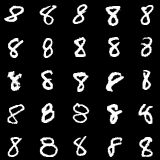
\includegraphics[width=\textwidth]{figures/einsum/mnist/[8]_ground_truth.png}
        \caption{Ground Truth}
    \end{subfigure}
    \begin{subfigure}[b]{0.24\textwidth}
        \centering
        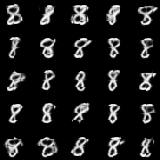
\includegraphics[width=\textwidth]{figures/einsum/mnist/[8]_EM.png}
        \caption{EM (LL: -15945)}
    \end{subfigure}
    \begin{subfigure}[b]{0.24\textwidth}
        \centering
        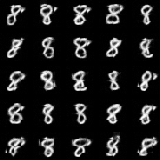
\includegraphics[width=\textwidth]{figures/einsum/mnist/[8]_SGD.png} 
        \caption{SGD (LL: -17796)}
    \end{subfigure}
    \begin{subfigure}[b]{0.24\textwidth}
        \centering
        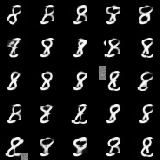
\includegraphics[width=\textwidth]{figures/einsum/mnist/[8]_SSM.png}
        \caption{SSM (LL: -22654)}
    \end{subfigure}
    \caption{Samples and Log-Likelihood of MNIST-class 8}
\end{figure}

\begin{figure}[H]
    \centering
    \begin{subfigure}[b]{0.24\textwidth}
        \centering
        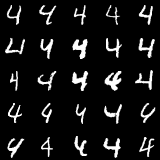
\includegraphics[width=\textwidth]{figures/einsum/mnist/[4]_ground_truth.png}
        \caption{Ground Truth}
    \end{subfigure}
    \begin{subfigure}[b]{0.24\textwidth}
        \centering
        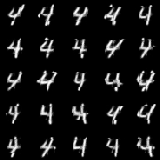
\includegraphics[width=\textwidth]{figures/einsum/mnist/[4]_EM.png}
        \caption{EM (LL: -13301)}
    \end{subfigure}
    \begin{subfigure}[b]{0.24\textwidth}
        \centering
        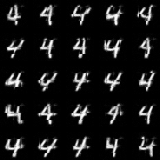
\includegraphics[width=\textwidth]{figures/einsum/mnist/[4]_SGD.png} 
        \caption{SGD (LL: -15626)}
    \end{subfigure}
    \begin{subfigure}[b]{0.24\textwidth}
        \centering
        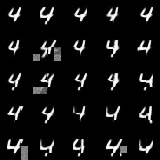
\includegraphics[width=\textwidth]{figures/einsum/mnist/[4]_SSM.png}
        \caption{SSM (LL: -20309)}
    \end{subfigure}
    \caption{Samples and Log-Likelihood of MNIST-class 4}
\end{figure}

Looking at these figures, specifically the NLL, we see a quite similar picture as in the 2D Density Estimation emerge. 
EM and SGD performed on par while SSM lagged a little behind. 
Also the time needed for training reflected the 2D counterpart, though the gap increased even more, meaning EM and SGD still took roughly the same while SSM now took roughly four times as long. 

When directly looking at the samples the results appear to be a bit different. While EM and SGD roughly provided the same samples, with SSM, they seemed to be the least "blurry" or most "clear", however with the caveat
that sometimes noisy artifacts appear, best scene with the 8 class. We also found that when introducing 
a weight decay in the optimizer, the number of these artifacts increase. Furthermore it often seemed that
one particular type of the provided digit dominated, meaning one weight in the mixture approaches $1$ while 
the others remain nearly at $0$ giving all samples a very similar look, best scene with the 7 class. \\

Finally we also performed image reconstructions, where a certain region of the image is masked out and then reconstructed using the trained model.
The masked out images as well as the reconstructions for the same MNIST digits can be seen below.

\begin{figure}[H]
    \centering
    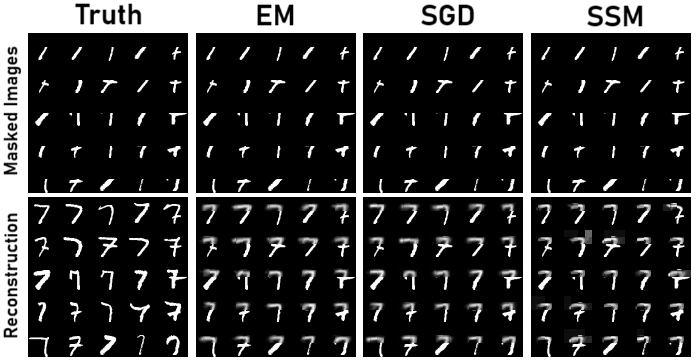
\includegraphics[width=\textwidth]{figures/einsum/mnist/reconstructions_7.png}
    \caption{Masked images and reconstructions of MNIST-class 7}
\end{figure}

\begin{figure}[H]
    \centering
    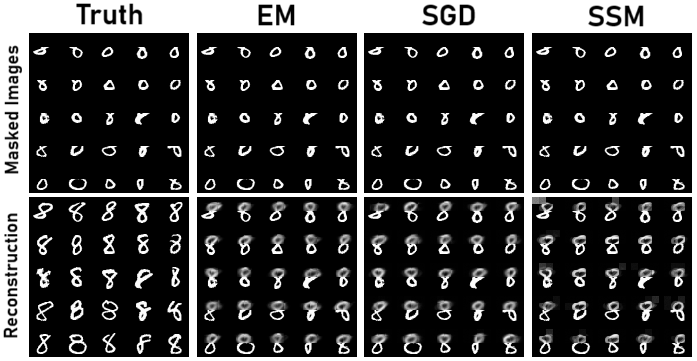
\includegraphics[width=\textwidth]{figures/einsum/mnist/reconstructions_8.png}
    \caption{Masked images and reconstructions of MNIST-class 8}
\end{figure}

\begin{figure}[H]
    \centering
    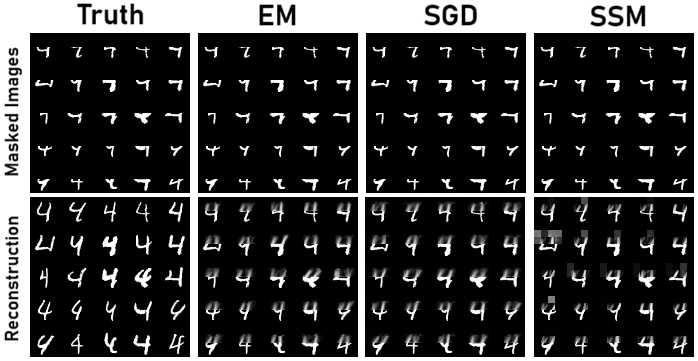
\includegraphics[width=\textwidth]{figures/einsum/mnist/reconstructions_4.png}
    \caption{Masked images and reconstructions of MNIST-class 4}
\end{figure}

\subsection{Multi Class Training}
\label{sec:exp_mnist_multi}


